% begin module sequence-squeeze-theorem
\begin{frame}
%The Squeeze Theorem also works for sequences:
\begin{theorem}[The Squeeze Theorem for Sequences]
If $\only<2->{\color{blue}} a_n\color{black}\leq \only<4->{\color{red}} b_n \color{black} \leq\only<3->{ \color{darkgreen}}c_n$ for $n \geq n_0$ and $\lim_{n\to\infty} a_n = L = \lim_{n\to\infty}c_n$, then $\alertNoH{5}{ \lim_{n\to\infty}b_n=L}$.
\end{theorem}
\psset{xunit=1cm, yunit=1cm}
\hfil
\begin{pspicture}(-0.5,-0.5)(10, 2.7)
\tiny
\fcBoundingBox{-0.5}{-0.5}{7}{2.9}
\fcAxesStandard{-0.5}{-0.5}{7}{2.6}%
\uncover<1,4->{%
\rput[b](0,2.65){$a$}%
\rput[l](7.1,0){$n$}%
}%
\uncover<handout:0|2,3>{%
\rput[b](0,2.7){$y$}%
\rput[l](7.1,0){$x$}%
}%
\multido{\na=1+1}{35}{%
\pstVerb{2 dict begin /na \na\space def /t na 0.2 mul def}%
\uncover<3->{\fcFullDot[scale=0.6, linecolor=darkgreen]{t }{1 t 1 add div 1 add}}%
\uncover<2->{\fcFullDot[scale=0.6, linecolor=blue]{t }{-1 t 1 add div 1 add}}%
\uncover<4->{\fcFullDot[scale=0.6, linecolor=red]{t }{1 t 1 add div t 180 mul sin mul 1 add}}%
\pstVerb{end}%
}%
\uncover<5->{\psline[linewidth =0.4pt, linestyle=dashed, linecolor=blue](0, 1)(7, 1)}
\rput[r](-0.1, 1){\uncover<5->{\alertNoH{5}{$L$}}}
\uncover<3-8>{\rput[b](0.2, 2){\color{darkgreen}$c_n$}}
\uncover<4-9>{\rput[t](0.2, 1.4){\color{red}$b_n$}}
\uncover<2-7>{\rput[b](0.2, 0.4){\color{blue}$a_n$}}

\uncover<handout:0|9->{\rput[lb](0.2, 2){\color{darkgreen}$h(x)$}}
\uncover<handout:0|10->{\rput[lt](0.2, 1.4){\color{red}$g(x)$}}
\uncover<handout:0|8->{\rput[lb](0.2, 0.4){\color{blue}$f(x)$}}

\uncover<handout:0|8->{\psplot[linecolor=blue, plotpoints=500]{0 }{7}{-1 x 1 add div 1 add}}%
\uncover<handout:0|9->{\psplot[linecolor=darkgreen, plotpoints=500]{0 }{7}{1 x 1 add div 1 add}}%
\uncover<handout:0|10->{\psplot[linecolor=red, plotpoints=500]{0 }{7}{1 x 1 add div x 180 mul sin mul 1 add}}%

\end{pspicture}
%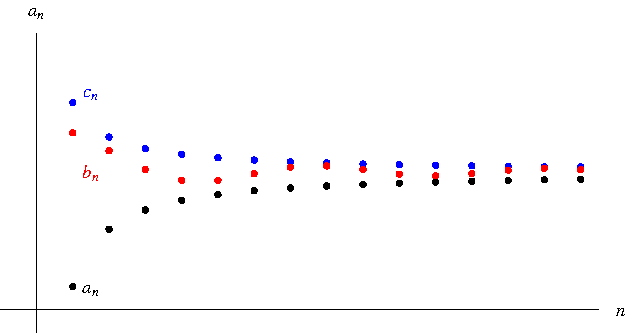
\includegraphics[width=8cm]{sequences/pictures/12-01-squeeze.pdf}%
\uncover<6->{%
%Here is a corollary to the Squeeze Theorem for sequences:
\begin{corollary}[to the squeeze theorem]
If $\lim_{n\to\infty} |a_n| = 0$, then $\lim_{n\to\infty}a_n = 0$.
\end{corollary}
}%

\uncover<7->{
\begin{theorem}[Squeeze theorem for functions at $\infty$]
If $\only<8->{\color{blue}}f(x)\color{black} \leq \only<10->{\color{red}} g(x)\color{black}\leq \only<9->{\color{darkgreen}} h(x)$ and $\lim_{x\to\infty} f(x) = L = \lim_{x\to\infty}g(x)$, then $\lim_{x\to\infty}f(x)=L$.
\end{theorem}
}
\end{frame}
% end module sequence-squeeze-theorem
